\documentclass{article}\usepackage[]{graphicx}\usepackage[]{color}
%% maxwidth is the original width if it is less than linewidth
%% otherwise use linewidth (to make sure the graphics do not exceed the margin)
\makeatletter
\def\maxwidth{ %
  \ifdim\Gin@nat@width>\linewidth
    \linewidth
  \else
    \Gin@nat@width
  \fi
}
\makeatother

\definecolor{fgcolor}{rgb}{0.345, 0.345, 0.345}
\newcommand{\hlnum}[1]{\textcolor[rgb]{0.686,0.059,0.569}{#1}}%
\newcommand{\hlstr}[1]{\textcolor[rgb]{0.192,0.494,0.8}{#1}}%
\newcommand{\hlcom}[1]{\textcolor[rgb]{0.678,0.584,0.686}{\textit{#1}}}%
\newcommand{\hlopt}[1]{\textcolor[rgb]{0,0,0}{#1}}%
\newcommand{\hlstd}[1]{\textcolor[rgb]{0.345,0.345,0.345}{#1}}%
\newcommand{\hlkwa}[1]{\textcolor[rgb]{0.161,0.373,0.58}{\textbf{#1}}}%
\newcommand{\hlkwb}[1]{\textcolor[rgb]{0.69,0.353,0.396}{#1}}%
\newcommand{\hlkwc}[1]{\textcolor[rgb]{0.333,0.667,0.333}{#1}}%
\newcommand{\hlkwd}[1]{\textcolor[rgb]{0.737,0.353,0.396}{\textbf{#1}}}%
\let\hlipl\hlkwb

\usepackage{framed}
\makeatletter
\newenvironment{kframe}{%
 \def\at@end@of@kframe{}%
 \ifinner\ifhmode%
  \def\at@end@of@kframe{\end{minipage}}%
  \begin{minipage}{\columnwidth}%
 \fi\fi%
 \def\FrameCommand##1{\hskip\@totalleftmargin \hskip-\fboxsep
 \colorbox{shadecolor}{##1}\hskip-\fboxsep
     % There is no \\@totalrightmargin, so:
     \hskip-\linewidth \hskip-\@totalleftmargin \hskip\columnwidth}%
 \MakeFramed {\advance\hsize-\width
   \@totalleftmargin\z@ \linewidth\hsize
   \@setminipage}}%
 {\par\unskip\endMakeFramed%
 \at@end@of@kframe}
\makeatother

\definecolor{shadecolor}{rgb}{.97, .97, .97}
\definecolor{messagecolor}{rgb}{0, 0, 0}
\definecolor{warningcolor}{rgb}{1, 0, 1}
\definecolor{errorcolor}{rgb}{1, 0, 0}
\newenvironment{knitrout}{}{} % an empty environment to be redefined in TeX

\usepackage{alltt}
\usepackage{natbib}



\IfFileExists{upquote.sty}{\usepackage{upquote}}{}
\begin{document}
\title {Romeo and Juliet Wordcloud}
\author {Jerrin Joe Varghese}
\maketitle


\begin{abstract}
In this article we are constructing a wordcloud using the tidytext R package.
Here we will be taking the words from the famous book Romeo and Juliets written by shakespear.
We will extract all the words and convert it to a cloud of words in different shape and colurs using the package wordcloud.
\end{abstract}

\textit{Romeo and Juliet} is a tragic love story written by  William Shakespeare early \noindent in his career.\footnote{The date of the publish is not available.}

\section {The Gutenberg Package}
This is a relatively new package for R,Gutenberg , that gives one access to all of the novels written by different authors.

\begin{knitrout}
\definecolor{shadecolor}{rgb}{0.969, 0.969, 0.969}\color{fgcolor}\begin{kframe}
\begin{alltt}
\hlkwd{library}\hlstd{(janeaustenr)}
\hlkwd{library}\hlstd{(dplyr)}
\hlkwd{library}\hlstd{(tidytext)}
\hlkwd{library}\hlstd{(gutenbergr)}
\hlkwd{library}\hlstd{(wordcloud)}
\hlkwd{library}\hlstd{(wordcloud2)}
\hlkwd{library}\hlstd{(ggplot2)}
\hlkwd{library}\hlstd{(stringr)}
\end{alltt}
\end{kframe}
\end{knitrout}


Let's find the book for Romeo and Juliets by shakespear using gutenberg.

\begin{knitrout}
\definecolor{shadecolor}{rgb}{0.969, 0.969, 0.969}\color{fgcolor}\begin{kframe}
\begin{alltt}
\hlkwd{gutenberg_works}\hlstd{(}\hlkwd{str_detect}\hlstd{(title,}\hlstr{'Romeo'}\hlstd{))}
\end{alltt}
\begin{verbatim}
## # A tibble: 3 x 8
##   gutenberg_id
##          <int>
## 1         1513
## 2        22274
## 3        47960
## # ... with 7 more variables: title <chr>, author <chr>,
## #   gutenberg_author_id <int>, language <chr>, gutenberg_bookshelf <chr>,
## #   rights <chr>, has_text <lgl>
\end{verbatim}
\end{kframe}
\end{knitrout}

Let's now download and store it into a data frame.

\begin{knitrout}
\definecolor{shadecolor}{rgb}{0.969, 0.969, 0.969}\color{fgcolor}\begin{kframe}
\begin{alltt}
\hlstd{Romeo}\hlkwb{<-}\hlkwd{gutenberg_download}\hlstd{(}\hlnum{1513}\hlstd{)}
\end{alltt}
\end{kframe}
\end{knitrout}


\section {Some Data Cleaning}

Adding a new column of line to get the line numbers and clean the id to Null.

\begin{knitrout}
\definecolor{shadecolor}{rgb}{0.969, 0.969, 0.969}\color{fgcolor}\begin{kframe}
\begin{alltt}
\hlstd{Romeo}\hlopt{$}\hlstd{line}\hlkwb{<-}\hlnum{1}\hlopt{:}\hlnum{5268}
\hlstd{Romeo}\hlopt{$}\hlstd{gutenberg_id}\hlkwb{<-}\hlkwa{NULL}
\end{alltt}
\end{kframe}
\end{knitrout}



\section{The wordcloud}
To make the word cloud, we first need to break up the lines into words. We can use the function from package tidytext for this.

\begin{knitrout}
\definecolor{shadecolor}{rgb}{0.969, 0.969, 0.969}\color{fgcolor}\begin{kframe}
\begin{alltt}
\hlstd{Romeo_words}\hlkwb{<-}\hlstd{Romeo}\hlopt
  \hlkwd{unnest_tokens}\hlstd{(word,text)}
\end{alltt}
\end{kframe}
\end{knitrout}

We can remove common, unimportant words with the stop\_words from the data frame with dplyr.
\begin{knitrout}
\definecolor{shadecolor}{rgb}{0.969, 0.969, 0.969}\color{fgcolor}\begin{kframe}
\begin{alltt}
\hlstd{Romeo_words}\hlkwb{<-}\hlstd{Romeo_words}\hlopt
  \hlkwd{filter}\hlstd{(}\hlopt{!}\hlstd{(word} \hlopt \hlstd{stop_words}\hlopt{$}\hlstd{word))}
\end{alltt}
\end{kframe}
\end{knitrout}


Since this is a tragic love story, so lets only take the joy and sadness word sentiments out of it.

\begin{knitrout}
\definecolor{shadecolor}{rgb}{0.969, 0.969, 0.969}\color{fgcolor}\begin{kframe}
\begin{alltt}
\hlstd{nrc}\hlkwb{<-}\hlkwd{get_sentiments}\hlstd{(}\hlstr{'nrc'}\hlstd{)}

\hlstd{joy_sad}\hlkwb{<-}\hlstd{nrc}\hlopt
  \hlkwd{filter}\hlstd{(sentiment} \hlopt{==} \hlstr{'joy'} \hlopt{|} \hlstd{sentiment} \hlopt{==} \hlstr{'sadness'}\hlstd{)}
\end{alltt}
\end{kframe}
\end{knitrout}

Lets takeout all the joy and sadness words to a dataframe.

\begin{knitrout}
\definecolor{shadecolor}{rgb}{0.969, 0.969, 0.969}\color{fgcolor}\begin{kframe}
\begin{alltt}
\hlstd{Romeo_joy_sad}\hlkwb{<-}\hlkwd{inner_join}\hlstd{(Romeo_words,joy_sad)}
\end{alltt}
\end{kframe}
\end{knitrout}

Now we need to calculate frequencies of the words in the novel.  Again, we can use standard techniques for this:

\begin{knitrout}
\definecolor{shadecolor}{rgb}{0.969, 0.969, 0.969}\color{fgcolor}\begin{kframe}
\begin{alltt}
\hlstd{Romeo_frequency}\hlkwb{<-}\hlstd{Romeo_joy_sad}\hlopt
  \hlkwd{group_by}\hlstd{(word)}\hlopt
  \hlkwd{summarise}\hlstd{(}\hlkwc{frequency} \hlstd{=} \hlkwd{n}\hlstd{())}
\end{alltt}
\end{kframe}
\end{knitrout}

Finally lets view our wordcloud.

\begin{knitrout}
\definecolor{shadecolor}{rgb}{0.969, 0.969, 0.969}\color{fgcolor}\begin{kframe}
\begin{alltt}
\hlkwd{wordcloud}\hlstd{(Romeo_frequency}\hlopt{$}\hlstd{word,Romeo_frequency}\hlopt{$}\hlstd{frequency)}
\end{alltt}
\end{kframe}
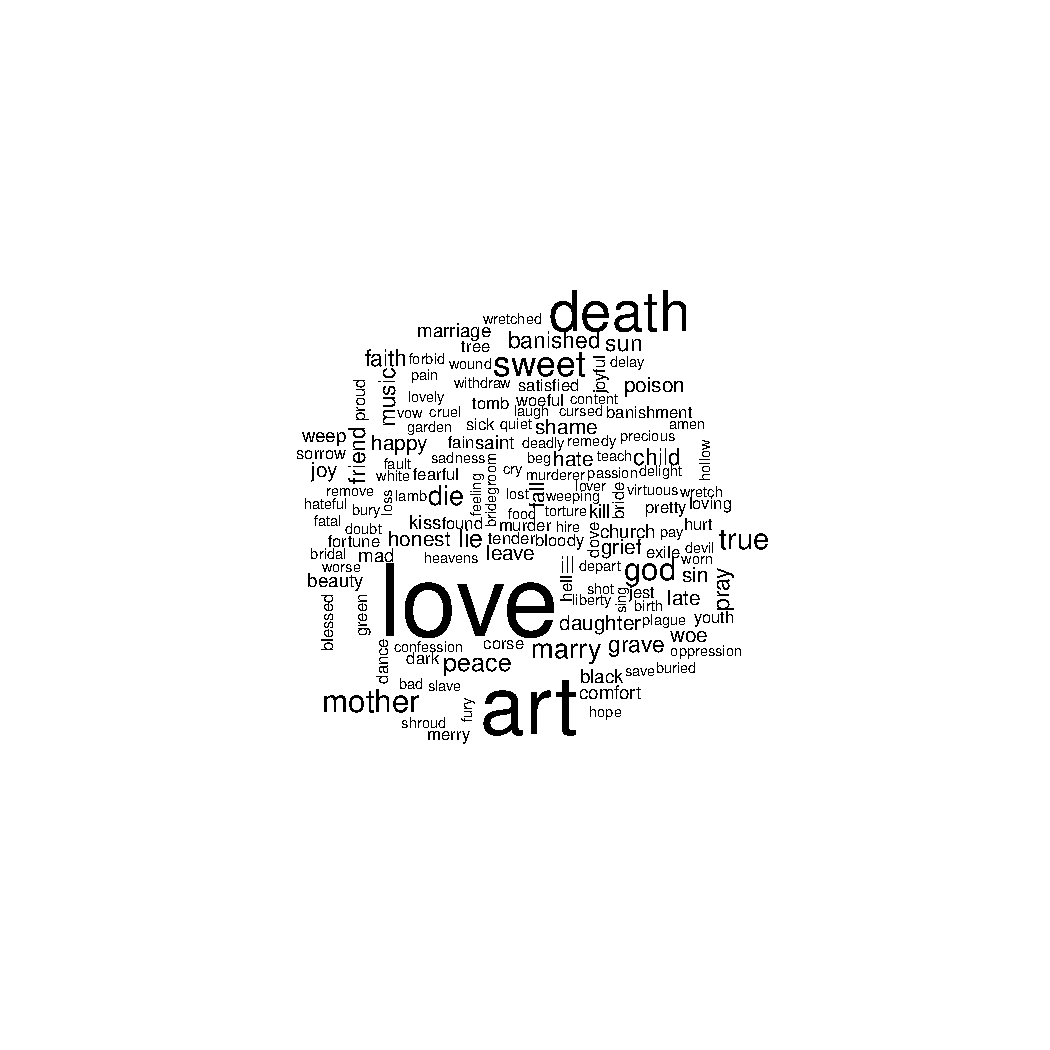
\includegraphics[width=\maxwidth]{figure/unnamed-chunk-11-1} 

\end{knitrout}




\section{Sentiment Afinn}

There is also another package afinn, which has 2 columns in its data frame, one with the sentiments and the other with the score for those words.
Let's look into it.

\begin{knitrout}
\definecolor{shadecolor}{rgb}{0.969, 0.969, 0.969}\color{fgcolor}\begin{kframe}
\begin{alltt}
\hlstd{affin}\hlkwb{<-}\hlkwd{get_sentiments}\hlstd{(}\hlstr{'afinn'}\hlstd{)}
\end{alltt}
\end{kframe}
\end{knitrout}

Next, we can also divide the lines into groups or chuncks.That we can do by using " %/% num ".Here we are dividing by 80.

\begin{knitrout}
\definecolor{shadecolor}{rgb}{0.969, 0.969, 0.969}\color{fgcolor}\begin{kframe}
\begin{alltt}
\hlstd{Romeo_words}\hlopt{$}\hlstd{groups}\hlkwb{<-}\hlstd{Romeo_words}\hlopt{$}\hlstd{line}\hlopt\hlnum{80}
\end{alltt}
\end{kframe}
\end{knitrout}


We can use inner_join to get our desired words from  the sentiments, this is a way of 
cleaning.

\begin{knitrout}
\definecolor{shadecolor}{rgb}{0.969, 0.969, 0.969}\color{fgcolor}\begin{kframe}
\begin{alltt}
\hlstd{Romeo_words}\hlkwb{<-}\hlkwd{inner_join}\hlstd{(Romeo_words,affin)}
\end{alltt}
\end{kframe}
\end{knitrout}


Now, lets score our words in groups of 80line that we have divided.


\begin{knitrout}
\definecolor{shadecolor}{rgb}{0.969, 0.969, 0.969}\color{fgcolor}\begin{kframe}
\begin{alltt}
\hlstd{Romeo_senti_score}\hlkwb{<-}\hlstd{Romeo_words}\hlopt
  \hlkwd{group_by}\hlstd{(groups)}\hlopt
  \hlkwd{summarise}\hlstd{(}\hlkwc{Romeo_score}\hlstd{=}\hlkwd{sum}\hlstd{(score))}
\end{alltt}
\end{kframe}
\end{knitrout}

Let us plot the graph for this score.
\begin{knitrout}
\definecolor{shadecolor}{rgb}{0.969, 0.969, 0.969}\color{fgcolor}\begin{kframe}
\begin{alltt}
\hlkwd{ggplot}\hlstd{()}\hlopt{+}
  \hlkwd{geom_point}\hlstd{(}\hlkwc{data}\hlstd{=Romeo_senti_score,}\hlkwd{aes}\hlstd{(}\hlkwc{x}\hlstd{=groups,}\hlkwc{y}\hlstd{=Romeo_score))}\hlopt{+}
  \hlkwd{geom_line}\hlstd{(}\hlkwc{data}\hlstd{=Romeo_senti_score,}\hlkwd{aes}\hlstd{(}\hlkwc{x}\hlstd{=groups,}\hlkwc{y}\hlstd{=Romeo_score))}
\end{alltt}
\end{kframe}
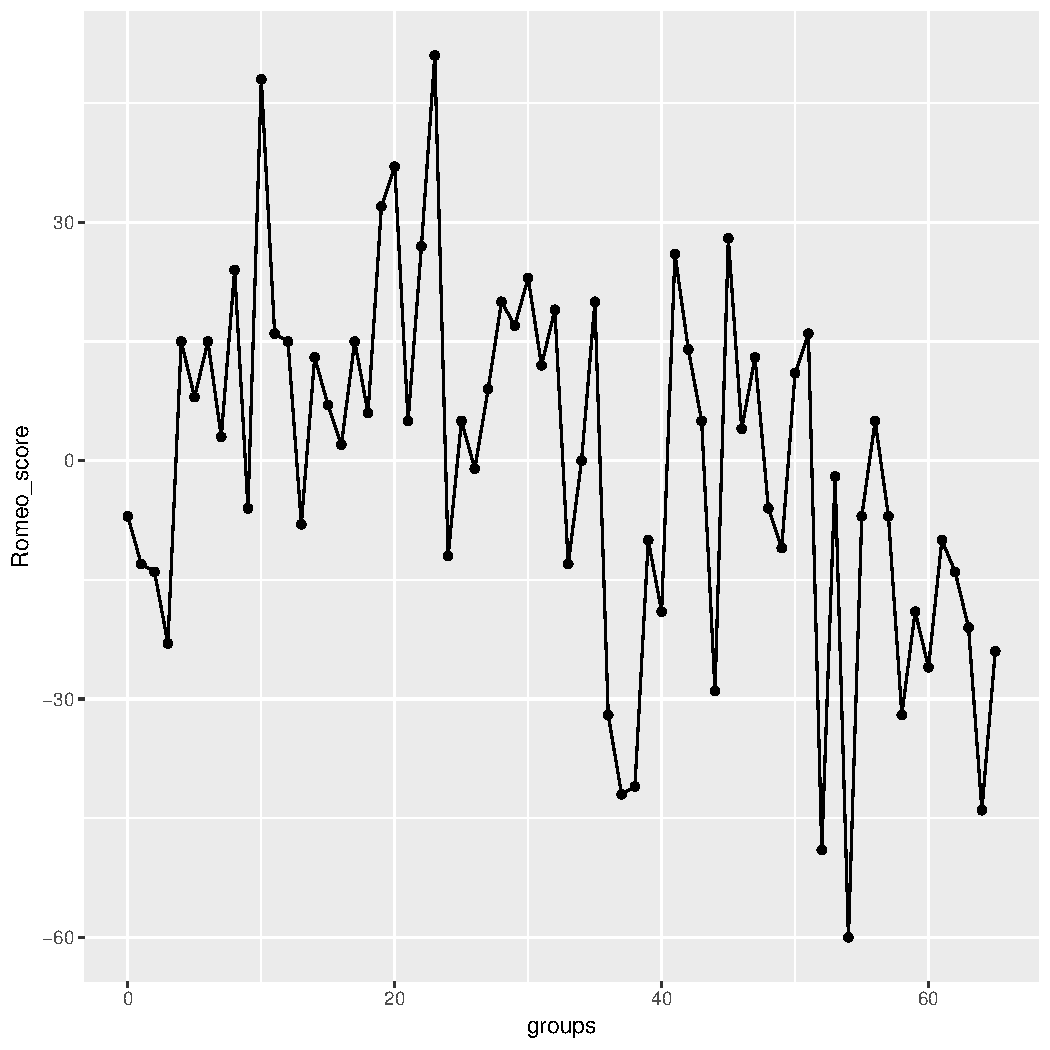
\includegraphics[width=\maxwidth]{figure/unnamed-chunk-16-1} 

\end{knitrout}


\bibliographystyle{apa}
\bibliography{romeo}
\nocite{*}
\end{document}
